        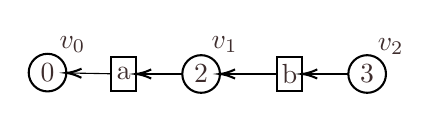
\begin{tikzpicture}[x=0.5pt,y=0.5pt,yscale=-1,xscale=1]
        %uncomment if require: \path (0,306); %set diagram left start at 0, and has height of 306


        % Text Node
        \draw  [line width=0.75]   (92, 109) circle [x radius= 13.6, y radius= 13.6]   ;
        \draw (92,109) node [color={rgb, 255:red, 62; green, 45; blue, 45 }  ,opacity=1 ]  {$0$};
        % Text Node
        \draw  [line width=0.75]   (138,98) -- (156,98) -- (156,122) -- (138,122) -- cycle  ;
        \draw (147,110) node [scale=1,color={rgb, 255:red, 62; green, 45; blue, 45 }  ,opacity=1 ]  {a};
        % Text Node
        \draw  [line width=0.75]   (203, 110) circle [x radius= 13.6, y radius= 13.6]   ;
        \draw (203,110) node [color={rgb, 255:red, 62; green, 45; blue, 45 }  ,opacity=1 ]  {$2$};
        % Text Node
        \draw (110,89) node [color={rgb, 255:red, 62; green, 45; blue, 45 }  ,opacity=1 ]  {$v_{0}$};
        % Text Node
        \draw (220,89) node [color={rgb, 255:red, 62; green, 45; blue, 45 }  ,opacity=1 ]  {$v_{1}$};
        % Text Node
        \draw  [line width=0.75]   (258,98) -- (276,98) -- (276,122) -- (258,122) -- cycle  ;
        \draw (267,110) node [scale=1,color={rgb, 255:red, 62; green, 45; blue, 45 }  ,opacity=1 ]  {b};
        % Text Node
        \draw  [line width=0.75]   (323, 110) circle [x radius= 13.6, y radius= 13.6]   ;
        \draw (323,110) node [color={rgb, 255:red, 62; green, 45; blue, 45 }  ,opacity=1 ]  {$3$};
        % Text Node
        \draw (340,90) node [color={rgb, 255:red, 62; green, 45; blue, 45 }  ,opacity=1 ]  {$v_{2}$};
        % Connection
        \draw    (138,109.84) -- (107.6,109.28) ;
        \draw [shift={(105.6,109.25)}, rotate = 361.03999999999996] [color={rgb, 255:red, 0; green, 0; blue, 0 }  ][line width=0.75]    (10.93,-3.29) .. controls (6.95,-1.4) and (3.31,-0.3) .. (0,0) .. controls (3.31,0.3) and (6.95,1.4) .. (10.93,3.29)   ;

        % Connection
        \draw    (189.4,110) -- (158,110) ;
        \draw [shift={(156,110)}, rotate = 360] [color={rgb, 255:red, 0; green, 0; blue, 0 }  ][line width=0.75]    (10.93,-3.29) .. controls (6.95,-1.4) and (3.31,-0.3) .. (0,0) .. controls (3.31,0.3) and (6.95,1.4) .. (10.93,3.29)   ;

        % Connection
        \draw    (309.4,110) -- (278,110) ;
        \draw [shift={(276,110)}, rotate = 360] [color={rgb, 255:red, 0; green, 0; blue, 0 }  ][line width=0.75]    (10.93,-3.29) .. controls (6.95,-1.4) and (3.31,-0.3) .. (0,0) .. controls (3.31,0.3) and (6.95,1.4) .. (10.93,3.29)   ;

        % Connection
        \draw    (258,110) -- (218.6,110) ;
        \draw [shift={(216.6,110)}, rotate = 360] [color={rgb, 255:red, 0; green, 0; blue, 0 }  ][line width=0.75]    (10.93,-3.29) .. controls (6.95,-1.4) and (3.31,-0.3) .. (0,0) .. controls (3.31,0.3) and (6.95,1.4) .. (10.93,3.29)   ;


        \end{tikzpicture}
